
	\subsubsection{Use-Case Instance - uciugStatisticCrisisInTime:ugCrisisInTime}
	
	The administrator click the button to open the statics so the system has to call the information for the number of the crises compared with the time and send it back to the Administrator so he can see it. 		  
	\begin{operationmodel}
	\addheading{usergoal Use-Case Instance}
	\adddoublerow{Instantiated Use Case}{ugCrisisInTime}
	\adddoublerow{Instance ID}{uciugStatisticCrisisInTime}
	
	\end{operationmodel} 

	
	Figure \ref{fig:lu.uni.lassy.excalibur.examples.icrash-RE-UC-uci-uciugStatisticCrisisInTime}
	The administrator click the button to open the statics so the system has to call the information for the number of the crises compared with the time and send it back to the Administrator so he can see it. 
	
	\begin{figure}[htbp]
	\begin{center}
	
	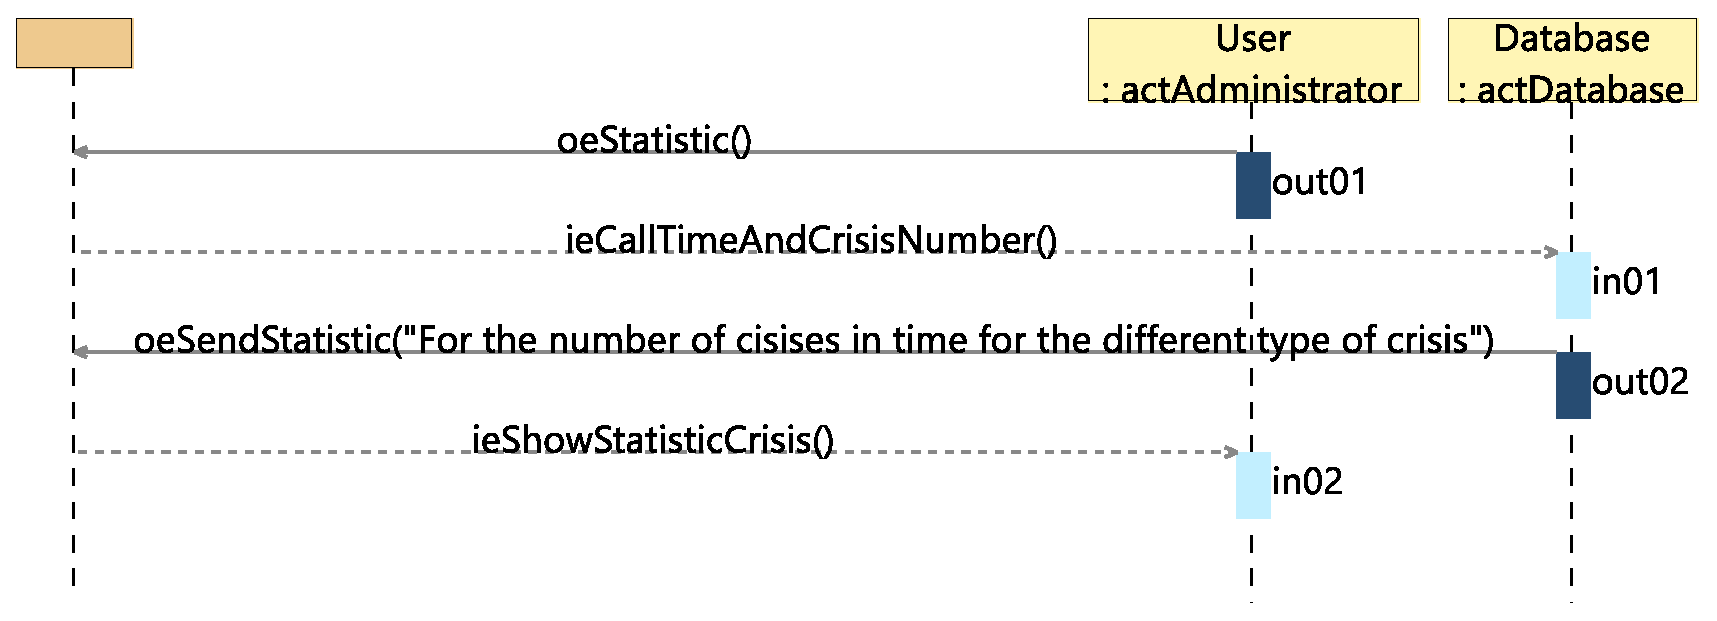
\includegraphics[
	angle=0
	,width=1.0\textwidth
	]{./images-report-gen/usecase-model/usergoal/uci-uciugStatisticCrisisInTime.eps}
	\end{center}
	\caption[lu.uni.lassy.excalibur.examples.icrash Sequence Diagram: uci-uciugStatisticCrisisInTime]{The number of the crises compared with the time}
	\label{fig:lu.uni.lassy.excalibur.examples.icrash-RE-UC-uci-uciugStatisticCrisisInTime}
	\end{figure}
	\vspace{0.5cm}
